\documentclass{article}

\usepackage{graphicx}
\usepackage{tikz}
\usepackage{tikzsymbols}
\usetikzlibrary{calc,patterns,shapes.geometric}
\pagestyle{empty}
\usepackage[margin=0pt]{geometry}
\geometry{papersize={14in,12in}}

\def\centerarc[#1](#2)(#3:#4:#5){\draw[#1] ($(#2)+({#5*cos(#3)},{#5*sin(#3)})$) arc (#3:#4:#5);}

\begin{document}
	\begin{figure}
		\centering
		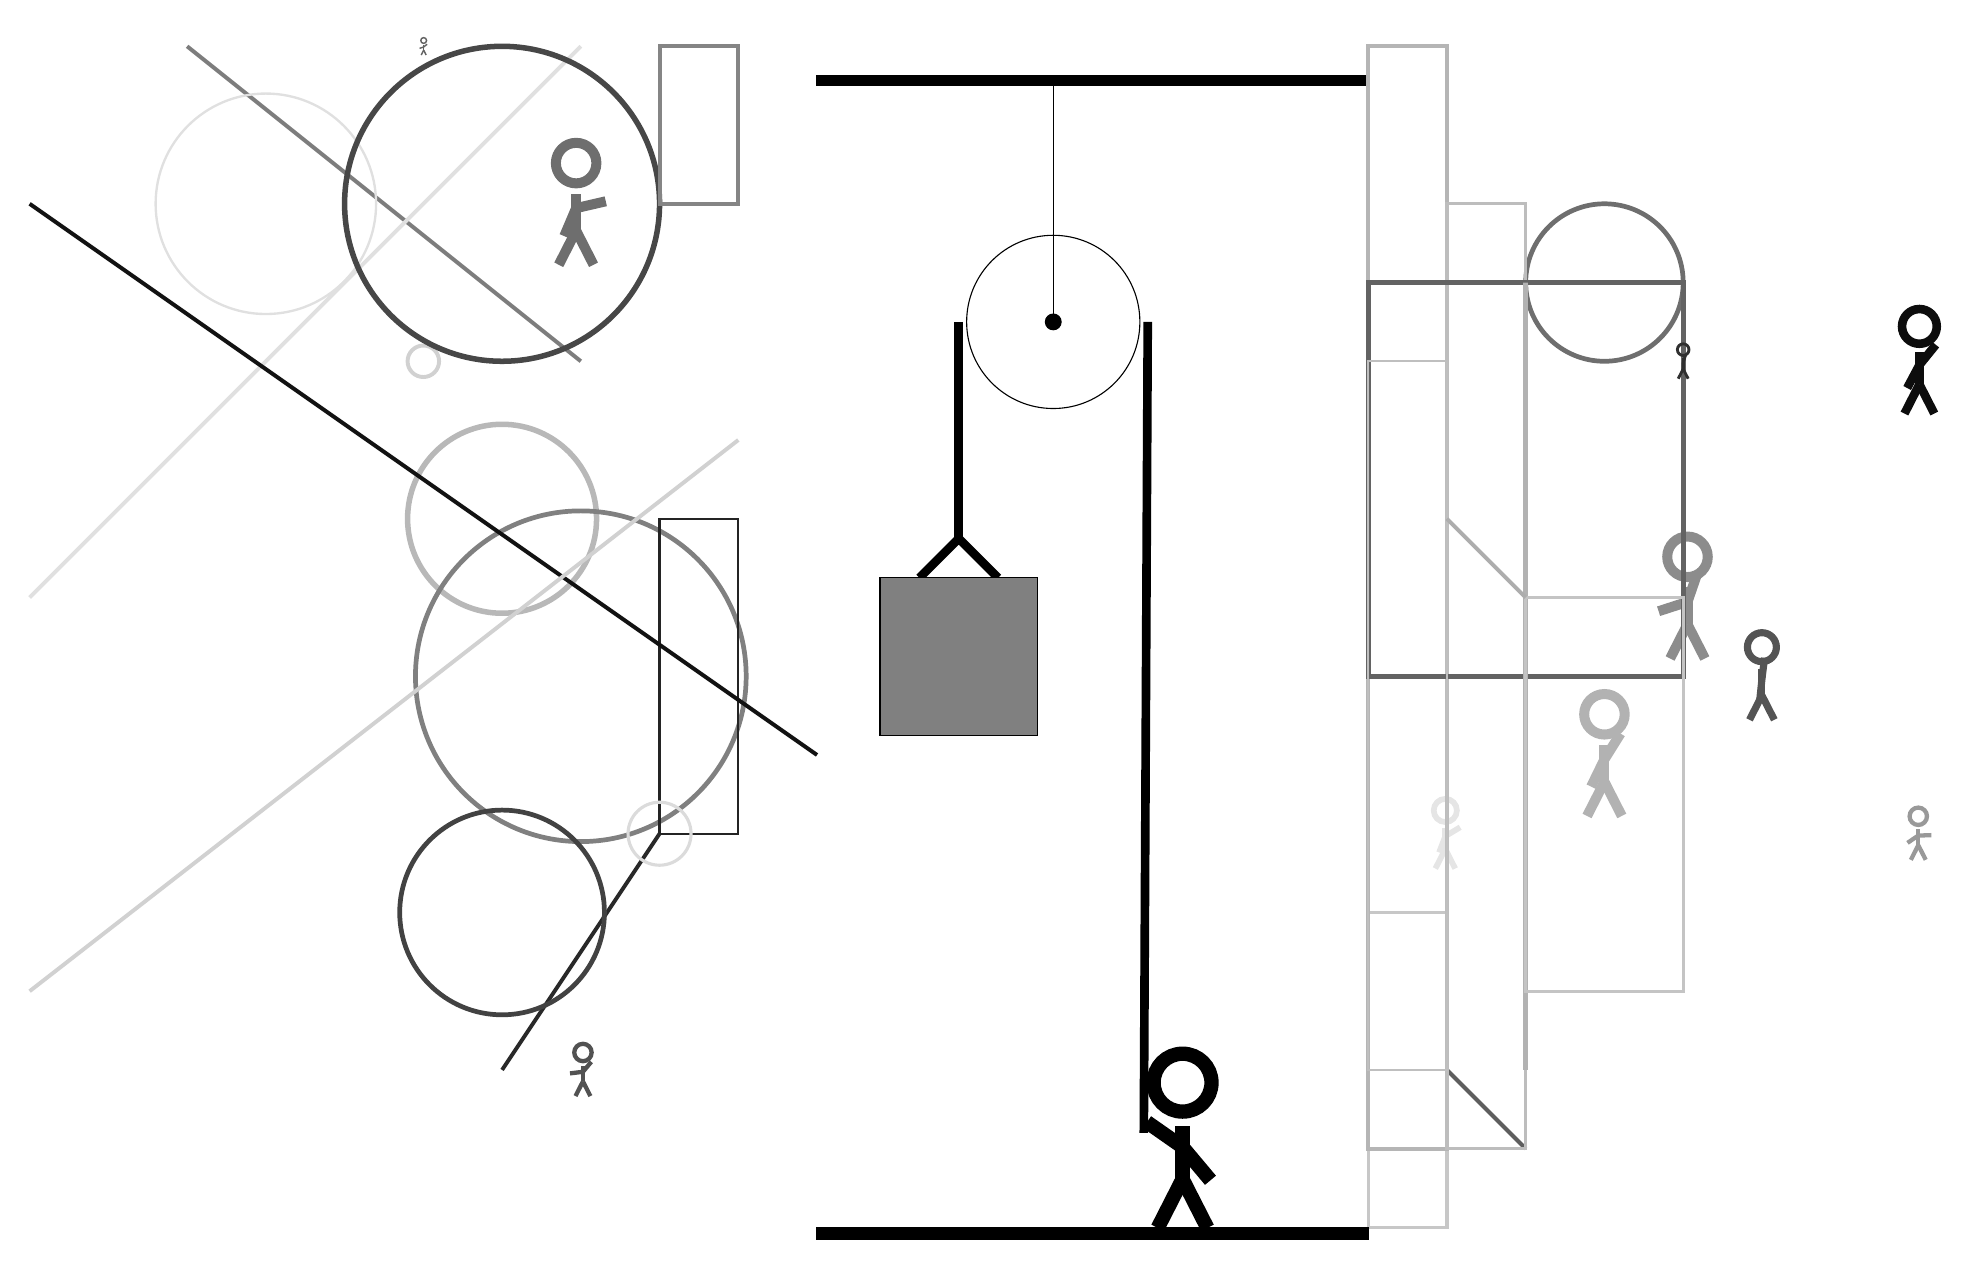
\begin{tikzpicture}
			%%%%% START %%%%%
			
			\draw[fill=black] (-2, 11.5) rectangle (5, 11.625);
			
			\draw (1, 8.5) circle (1.1);
			\draw[fill=black] (1, 8.5) circle (0.1);
			\draw (1, 11.5) -- (1, 8.5);
			
			\draw[line width=0.4mm, color=black!22] (5, -3) rectangle (6, 1);
			
			\draw [line width=0.7mm, color=black!28](-6, 6) circle (1.2);
			\node[line width=0.3mm, color=black!30] at (8, 3) {\Strichmaxerl[7][64][58]};
			\node[line width=0.5mm, color=black!10] at (6, 2) {\Strichmaxerl[4][69][31]};
			
			\draw [line width=0.5mm, color=black!18](-7, 8) circle (0.2);
			
			\draw [line width=0.6mm, color=black!50](-5, 4) circle (2.1);
			\draw[line width=0.4mm, color=black!10] (5, 4) rectangle (5, 3);
			\node[line width=0.4mm, color=black!95] at (12, 8) {\Strichmaxerl[6][62][51]};
			\node[line width=0.4mm, color=black!61] at (-7, 12) {\Strichmaxerl[1][19][38]};
			\draw [line width=0.6mm, color=black!57](8, 9) circle (1.0);
			\draw[line width=0.3mm, color=black!86] (-4, 6) rectangle (-3, 2);
			\draw [line width=0.4mm, color=black!28](-10, 3) circle (0.0);
			\node[line width=0.2mm, color=black!57] at (-5, 10) {\Strichmaxerl[7][67][13]};
			
			\draw[line width=0.5mm, color=black!63](6, -1) -- (7, -2);
			\draw[line width=0.5mm, color=black!51](-5, 8) -- (-10, 12);
			\draw[line width=0.5mm, color=black!29] (6, -2) rectangle (5, 12);
			\draw[line width=0.4mm, color=black!26] (7, -2) rectangle (6, 10);
			
			\draw[line width=0.5mm, color=black!84](-6, -1) -- (-4, 2);
			\node[line width=0.6mm, color=black!67] at (10, 4) {\Strichmaxerl[5][84][83]};
			
			\node[line width=0.7mm, color=black!45] at (9, 5) {\Strichmaxerl[7][18][71]};
			\node[line width=0.2mm, color=black!68] at (-5, -1) {\Strichmaxerl[3][7][50]};
			
			\draw[line width=0.6mm, color=black!61] (5, 4) rectangle (9, 9);
			\draw [line width=0.3mm, color=black!12](-9, 10) circle (1.4);
			\draw [line width=0.4mm, color=black!14](-4, 2) circle (0.4);
			\draw [line width=0.6mm, color=black!74](-6, 1) circle (1.3);
			
			\draw[line width=0.5mm, color=black!12](-5, 12) -- (-12, 5);
			\draw[line width=0.6mm, color=black!30] (7, -1) rectangle (7, 9);
			\draw [line width=0.7mm, color=black!72](-6, 10) circle (2.0);
			\node[line width=0.4mm, color=black!81] at (9, 8) {\Strichmaxerl[2][88][72]};
			\draw[line width=0.2mm, color=black!25] (6, -1) rectangle (5, 8);
			\draw[line width=0.4mm, color=black!23] (7, 5) rectangle (9, 0);
			
			\draw[line width=0.5mm, color=black!48] (-3, 12) rectangle (-4, 10);
			\draw[line width=0.5mm, color=black!93](-2, 3) -- (-12, 10);
			\draw[line width=0.5mm, color=black!32](7, 5) -- (6, 6);
			\node[line width=0.5mm, color=black!40] at (12, 2) {\Strichmaxerl[3][34][2]};
			\draw[line width=0.5mm, color=black!18](-3, 7) -- (-12, 0);
			
			\draw[line width=1.1mm] (-0.7, 5.25) -- (-0.2, 5.75) -- (0.3, 5.25);
			\draw[fill=black!50] (-1.2, 5.25) rectangle (0.8, 3.25);
			
			\draw[line width=1.1mm] (-0.2, 8.5) -- (-0.2, 5.75);
			\centerarc[line width=1.1mm](1, 8.5)(0:180:1.2000000000000002);
			\draw[line width=1.1mm](2.2, 8.5) -- (2.15, -1.8);
			
			\node at (2.6, -1.9) {\Strichmaxerl[10][-35][-50]};
			
			\draw[fill=black] (-2, -3) rectangle (5, -3.15);
			
			%%%%% END %%%%%
		\end{tikzpicture}
	\end{figure}	
\end{document}